Für ein reibungsfreies Pendel mit Masse $m$ und Fadenlänge $l$ wirkt die Gewichtskraft
$\vec{F} = m \cdot \vec{a}$ der Bewegung entgegen. Dabei wird ein Drehmoment
$M = D_\su{p} \cdot \phi$ auf das Pendel ausgeübt. $\phi$ beschreibt den Auslenkwinkel
und $D_\su{p}$ ist die Winkelrichtgröße. Für die Bewegungsgleichung folgt damit die
Gleichung
\begin{equation}
  J \cdot \ddot{\phi} + D_\su{p}\phi = 0
\end{equation}
mit $J$ als Trägheitsmoment - mit der kleinen Winkelnäherung $\sin{(\phi)} = \phi$.
Für die Schwingungsfrequenz dieser harmonsichen Schwingung ergibt sich damit
\begin{equation}
  \omega = \sqrt{\frac{D_\su{p}}{J}} = \sqrt{\frac{g}{l}}.
\end{equation}
Somit ist die Schwingungsdauer weder von der Masse, noch vom Auslenkwinkel abhängig.

Werden zwei identische Pendel durch eine Feder miteinander gekoppelt, so wirkt
auf jedes Pendel ein zusätzliches Drehmoment $M_1 = D_\su{F}(\phi_2-\phi_1)$
bzw. $M_2 = D_\su{F}(\phi_1-\phi_2)$. Diese Bewegung lässt sich durch das System
folgender Differentialgleichungen darstellen:
\begin{align}
  J \ddot{\phi_1} + D\phi_1 &= D_\su{F} (\phi_2-\phi1) \\
  J \ddot{\phi_2} + D\phi_2 &= D_\su{F} (\phi_1\phi2) .
\end{align}
Die linke Seite beschreibt die Schwingung des einzelnen Pendels, die rechte Seite
berücktsichtigt die Kopplung der Feder.
Dieses System lässt sich in zwei einzelne Eigenschwingungen zerlegen, welche
harmonische Schwingungen mit den Frequenzen $\omega_1$ und $\omega_2$ und den Auslenkwinkeln
$\alpha_1$ und $\alpha_2$ darstellen.

Durch die Anfangsbesdingungen $\alpha (t=0)$ und $\dot{\alpha}(t=0)$ entstehen drei verschiedene
Schwingungsarten.
Zum einen gibt es die gleichsinnige Schwingung bei der $\alpha_1 = \alpha_2$ gilt.
\begin{figure}
  \centering
  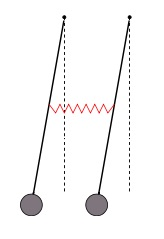
\includegraphics[width= 0.3\textwidth]{bilder/gleichsinnig.jpg}
  \caption{Gleichsinnige Schwingung\,\cite{106}}
\end{figure}
Dabei übt die Kopplungsfeder keine Kraft auf die Pendel aus, wodurch sie auch weggelassen
werden kann. Die Pendel schwingen somit in der Eigenfrequenz
\begin{equation}
  \omega_+ = \sqrt{\frac{g}{l}}
  \label{eqn:w+}.
\end{equation}
Die Schwingungsdauer $T$ beträgt dabei
\begin{equation}
  T_+ = 2 \pi \cdot \sqrt{\frac{l}{g}}
  \label{eqn:T+}.
\end{equation}
\par
Zum anderen gibt es die gegensinnige Schwingung mit $\alpha_1 = -\alpha_2$.
\begin{figure}
  \centering
  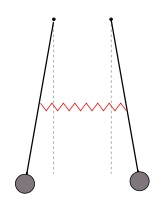
\includegraphics[width= 0.3\textwidth]{bilder/gegensinnig.jpg}
  \caption{Gegensinnige Schwingung\,\cite{106}}
\end{figure}
Dabei übt die Feder auf beide Pendel die gleiche Kraft aus, wodurch sich eine symmetrische
Schwingung mit der Frequenz
\begin{equation}
  \omega_-= \sqrt{\frac{g}{l}+\frac{2K}{l}}
  \label{eqn:w-}
\end{equation}
ergibt. Die Schwingungsdauer lautet
\begin{equation}
  T_-= 2\pi\sqrt{\frac{l}{g+2K}}
  \label{eqn:T-}
\end{equation}
mit $K$ als Kopplungskonstante der Feder.
\par
Abschließend gibt es die gekoppelte Schwingung mit $\alpha_1 = 0$ und $\alpha_2 ≠ 0$.
\begin{figure}
  \centering
  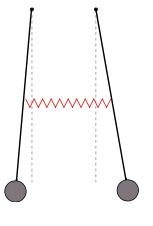
\includegraphics[width= 0.3\textwidth]{bilder/gekoppelte.jpg}
  \caption{Gekoppelte Schwingung\,\cite{106}}
\end{figure}
Zu Beginn befindet sich ein Pendel 1 in Ruhe und nur Pendel 2 wird ausgelenkt.
Beim Schwingen des zweiten Pendels wird die Energie auf das erste Pendel übertragen
und dieses beginnt langsam zu schwingen, die Amplitude nimmt dabei zu. Das Maximum wird
erreicht, wenn das zweite Pendel in Ruhe steht. Bei diesem Vorgang wird die Energie,
im Idealfall, vollständig übertragen, wodurch sich der Vorgang immer wieder wiederholt.
"Die Zeit zwischen zwei Stillständen eines Pendels wird Schwebung genannt" \cite{106}.
Die Schwebungsdauer $T_\su{S}$ ergibt sich durch
\begin{equation}
  T_\su{S} = \frac{T_+ \cdot T_-}{T_+ - T_-}
  \label{eqn:Ts}.
\end{equation}
Die Schwebungsfrequenz $\omega_\su{S}$ folgt durch
\begin{equation}
  \omega_\su{S} = \omega_+ - \omega_-  .
  \label{eqn:ws}
\end{equation}
Diese zwei Größen ergeben sich somit aus der gleichsinnigen und der gegensinnigen
Schwingung.

Die Kopplungskonstante $K$ wird als
\begin{equation}
  K = \frac{\omega_-^2 - \omega_+^2}{\omega_-^2 + \omega_+^2} = \frac{T_+^2 - T_-^2}{T_+^2 + T_-^2}
  \label{eqn:K}
\end{equation}
definiert.
